\documentclass[12pt]{article}
\setlength{\oddsidemargin}{0in}
\setlength{\evensidemargin}{0in}
\setlength{\textwidth}{6.5in}
\setlength{\parindent}{0in}
\setlength{\parskip}{\baselineskip}

\usepackage{amsmath,amsfonts,amssymb,bm,graphics,pgfplots,framed,dsfont,tikz}
\usepackage[scale=0.75,top=1cm,bottom=3cm]{geometry}
\usepackage[dvipsnames]{xcolor}

\begin{document}

\textbf{Minh Anh Nguyen }\\
\textbf{Discrete Mathematics\hfill Assignment-4}

\hrulefill

Section 2.1:

\begin{enumerate}
  \item Consider the following undirected graph.
  \begin{center}
    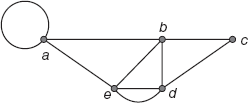
\includegraphics{img/img-0.png}
  \end{center}
  
        \begin{enumerate}
          \item How many edges are there in this graph?
          \begin{center}
            There are 9 edges in this graph.
          \end{center}
          
        
          \item Give the degree of each vertex.\\
          The dergree of each vertex is:
          \begin{center}
            a has degree 4\\
            b has degree 4\\
            c has degree 2\\
            d has degree 4\\
            e has degree 4\\
          \end{center}

          \item Do these numbers agree with Euler’s first observation? \\
          The sum of the degrees is 4 + 4 + 2 + 4 + 4 = 18. \\
          There are 9 edges in the graph. \\
          The sum of the degrees is doubled the number of edges.\\
          Hence, these numbers agree with Euler's first observation.
        \end{enumerate}

  \item Consider the following directed graph.
        \begin{center}
          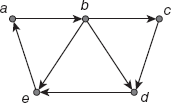
\includegraphics{img/img-1.png}
        \end{center}
        \begin{enumerate}
        \newpage
          \item Give the indegree of each vertex.\\
            \begin{center}
              The indegree of a is 1.\\
              The indegree of b is 1.\\
              The indegree of c is 1.\\
              The indegree of d is 2.\\
              The indegree of e is 2.
            \end{center}

          \item Give the outdegree of each vertex.\\
            \begin{center}
              The outdegree of a is 1.\\
              The outdegree of b is 3.\\
              The outdegree of c is 1.\\
              The outdegree of d is 1.\\
              The outdegree of e is 1.
            \end{center}

            \item Compute the sum of the indegrees and the sum of the outdegrees. What do you notice?\\
            The sum of the indegrees is:
            \[1 + 1 + 1 + 2 + 2 = 7\]
            The sum of the outdegrees is:
            \[1+3+1+1+1 = 7\]
            I noticed that the sum of the indegrees is equal to the sum of outdegrees and also equal to the numbers of edges.
            
        \end{enumerate}

  \item A circuit is \textit{simple} if it has no repeated edges. Draw a connected, undirected graph with seven vertices and no simple circuits. How many edges does it have?
  \begin{center}
    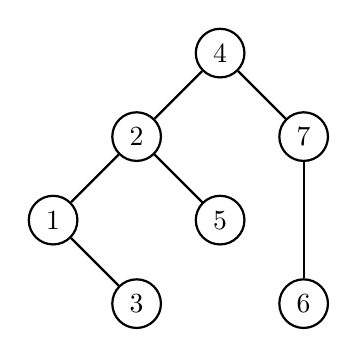
\begin{tikzpicture}[node distance={15mm}, thick, main/.style = {draw, circle}] 
      \node[main] (1) {$1$}; 
      \node[main] (2) [above right of=1] {$2$}; 
      \node[main] (3) [below right of=1] {$3$}; 
      \node[main] (4) [above right of=2] {$4$}; 
      \node[main] (5) [below right of=2] {$5$}; 
      \node[main] (6) [below right of=5] {$6$}; 
      \node[main] (7) [below right of=4] {$7$}; 
      \draw (1) -- (2); 
      \draw (1) -- (3); 
      \draw (2) -- (4); 
      \draw (2) -- (5);
      \draw (7) -- (6);
      \draw (4) -- (7);
      \end{tikzpicture} 
  \end{center}
  It has 6 edges.
  \newpage
  \item Draw an undirected graph with six vertices, each of degree 3, such that the graph is:
  \begin{enumerate}
    \item Connected.
    \begin{center}
      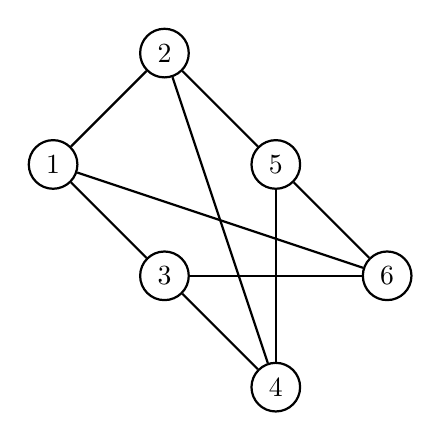
\begin{tikzpicture}[node distance={20mm}, thick, main/.style = {draw, circle}] 
        \node[main] (1) {$1$}; 
        \node[main] (2) [above right of=1] {$2$}; 
        \node[main] (3) [below right of=1] {$3$}; 
        \node[main] (4) [below right of=3] {$4$}; 
        \node[main] (5) [below right of=2] {$5$}; 
        \node[main] (6) [below right of=5] {$6$}; 
        \draw (1) -- (2); 
        \draw (1) -- (3); 
        \draw (3) -- (4);
        \draw (5) -- (4);
        \draw (2) -- (5);
        \draw (1) -- (6);
        \draw (3) -- (6);
        \draw (5) -- (6);
        \draw (4) -- (2);
        \end{tikzpicture} 
    \end{center}
    \item Not connected.
    \begin{center}
      \begin{tikzpicture}[node distance={15mm}, thick, main/.style = {draw, circle}] 
        \node[main] (1) {$1$}; 
        \node[main] (2) [above right of=1] {$2$}; 
        \node[main] (3) [above of=4] {$3$}; 
        \node[main] (4) [below right of=3] {$4$}; 
        \node[main] (5) [below left of=3] {$5$}; 
        \node[main] (6) [below left of=4] {$6$};
        \draw (1) to [out=180,in=270,looseness=5] (1); 
        \draw (2) to [out=0,in=90,looseness=5] (2); 
        \draw (1) -- (2);
        \draw (3) -- (4);
        \draw (3) -- (5);
        \draw (6) -- (5);
        \draw (6) -- (4);
        \draw (6) -- (3);
        \draw (5) -- (4);
        \end{tikzpicture} 
    \end{center}
  \end{enumerate}~\\
  \item A graph is called simple if it has no multiple edges or loops. Draw five different connected, simple, undirected graphs with four vertices.\\
  1.
  \begin{center}
    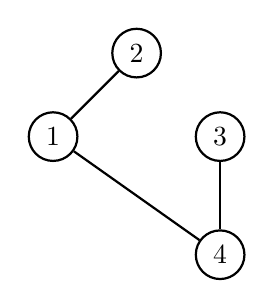
\begin{tikzpicture}[node distance={15mm}, thick, main/.style = {draw, circle}] 
      \node[main] (1) {$1$}; 
      \node[main] (2) [above right of=1] {$2$}; 
      \node[main] (3) [below right of=2] {$3$}; 
      \node[main] (4) [below of=3] {$4$}; 
      \draw (1) -- (2);
      \draw (1) -- (4);
      \draw (3) -- (4);
      \end{tikzpicture} 
  \end{center}
  \newpage
  2.
  \begin{center}
    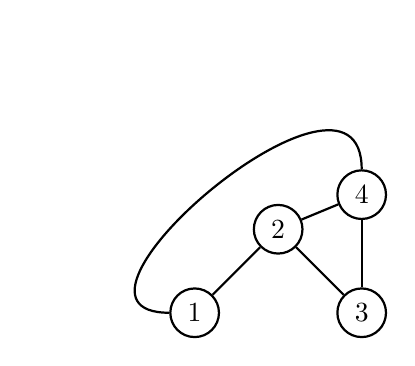
\begin{tikzpicture}[node distance={15mm}, thick, main/.style = {draw, circle}] 
      \node[main] (1) {$1$}; 
      \node[main] (2) [above right of=1] {$2$}; 
      \node[main] (3) [below right of=2] {$3$}; 
      \node[main] (4) [above of=3] {$4$}; 
      \draw (1) -- (2);
      \draw (3) -- (4);
      \draw (2) -- (3);
      \draw (2) -- (4);
      \draw (1) to [out=180,in=90,looseness=1.5] (4);
      \end{tikzpicture} 
  \end{center}
  3.
  \begin{center}
    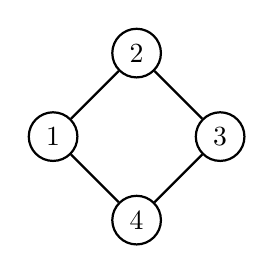
\begin{tikzpicture}[node distance={15mm}, thick, main/.style = {draw, circle}] 
      \node[main] (1) {$1$}; 
      \node[main] (2) [above right of=1] {$2$}; 
      \node[main] (3) [below right of=2] {$3$}; 
      \node[main] (4) [below right of=1] {$4$}; 
      \draw (1) -- (2);
      \draw (2) -- (3);
      \draw (3) -- (4);
      \draw (1) -- (4);
      \end{tikzpicture} 
  \end{center}
  4.
  \begin{center}
    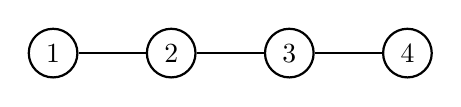
\begin{tikzpicture}[node distance={15mm}, thick, main/.style = {draw, circle}] 
      \node[main] (1) {$1$}; 
      \node[main] (2) [right of=1] {$2$}; 
      \node[main] (3) [right of=2] {$3$}; 
      \node[main] (4) [right of=3] {$4$}; 
      \draw (1) -- (2);
      \draw (2) -- (3);
      \draw (3) -- (4);
      \end{tikzpicture} 
  \end{center}
  5.
  \begin{center}
    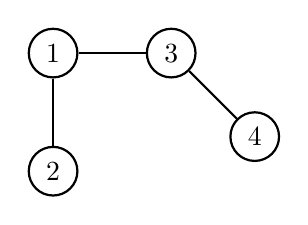
\begin{tikzpicture}[node distance={15mm}, thick, main/.style = {draw, circle}] 
      \node[main] (1) {$1$}; 
      \node[main] (2) [below of=1] {$2$}; 
      \node[main] (3) [right of=1] {$3$}; 
      \node[main] (4) [below right of=3] {$4$}; 
      \draw (1) -- (2);
      \draw (1) -- (3);
      \draw (3) -- (4);
      \end{tikzpicture} 
  \end{center}
  \item An undirected graph is called \textit{complete} if every vertex shares an edge with every other vertex. Draw a complete graph on five vertices. How many edges does it have?\\
  \begin{center}
    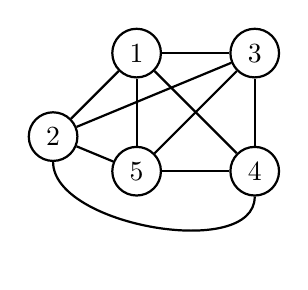
\begin{tikzpicture}[node distance={15mm}, thick, main/.style = {draw, circle}] 
      \node[main] (1) {$1$}; 
      \node[main] (2) [below left of=1] {$2$}; 
      \node[main] (3) [right of=1] {$3$}; 
      \node[main] (4) [below of=3] {$4$}; 
      \node[main] (5) [below of=1] {$5$}; 
      \draw (1) -- (2);
      \draw (1) -- (3);
      \draw (3) -- (4);
      \draw (2) -- (5);
      \draw (2) to [out=270, in=270, looseness=0.8] (4);      
      \draw (4) -- (5);
      \draw (1) -- (4);
      \draw (1) -- (5);
      \draw (2) -- (3);
      \draw (5) -- (3);
      \end{tikzpicture} 
  \end{center}
  It has 10 edges.
\end{enumerate}

\newpage
  Section 2.2:
\begin{enumerate}
  \item Draw Venn diagrams to illustrate De Morgan’s laws for sets (Theorem 2.1).\\~\\
    1. $(A \cup B)' =  A' \cap B'$
    \begin{center}
      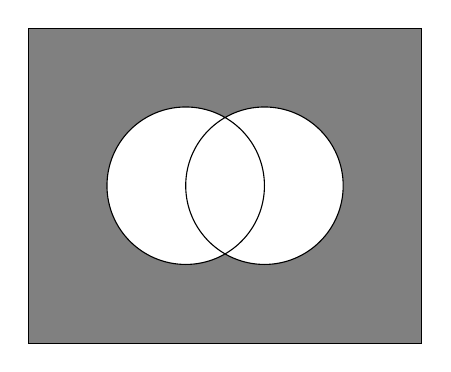
\begin{tikzpicture}
        \filldraw[fill=gray] (-2,-2) rectangle (3,2);
        
        % A \cap B (First circle)
        \scope
        \clip (0,0) circle (1);
        \fill[white] (0,0) circle (1);
        \endscope
    
        % Second circle filled with white
        \scope
        \clip (1,0) circle (1);
        \fill[white] (1,0) circle (1);
        \endscope
        
        % outline of both circles
        \draw (0,0) circle (1)
              (1,0) circle (1);
      \end{tikzpicture}
    \end{center}
    2. $(A \cap B)' = A' \cup B'$   
    \begin{center}
      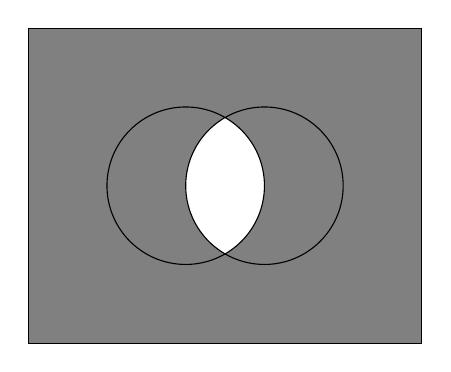
\begin{tikzpicture}
        \filldraw[fill=gray] (-2,-2) rectangle (3,2);
        
        % A \cap B (First circle)
        \scope
        \clip (1,0) circle (1);
        \fill[white] (0,0) circle (1);
        \endscope
    
        
        % outline of both circles
        \draw (0,0) circle (1)
              (1,0) circle (1);
      \end{tikzpicture}
    \end{center}
  \item Draw a Venn diagram to show the region $A \cap B'$. This region is also denoted $A \setminus B$, and is called the set difference.
    \begin{center}
      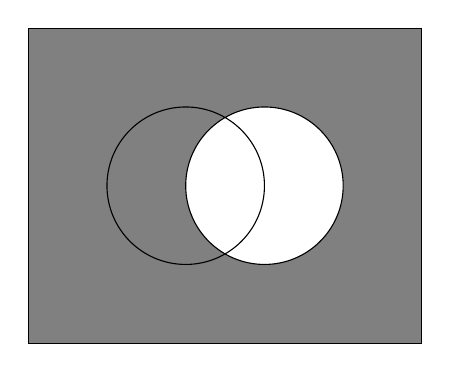
\begin{tikzpicture}
        \filldraw[fill=gray] (-2,-2) rectangle (3,2);
        
        % A \cap B (First circle)
        \scope
        \clip (0,0) circle (2);
        \fill[white] (1,0) circle (1);
        \endscope
    
        
        % outline of both circles
        \draw (0,0) circle (1)
              (1,0) circle (1);
      \end{tikzpicture}
    \end{center}
  \item Let $A = \{2, 3, 4\}$, $B = \{3, 4, 5, 6\}$, and suppose the universal set is $U = \{1, 2, …, 9\}$. List all the elements in the following sets.
  \begin{enumerate}
    \item $(A \cup B)' = \{1,7,8,9\}$
    \item $(A \cap B) \times A = \{3,4\} \times A = \{(3,2),(3,3)(3,4),(4,2),(4,3),(4,4)\}$ 
    \item $P(B\setminus A) = \{\phi, \{4\}, \{5\}, \{4,5\}\}$
  \end{enumerate}
  \newpage
  \item Let the following sets be given.
  \begin{center}
    C = the set of all charitable people.\\
    G = the set of all good citizen.\\
    P = the set of all polite people.\\
  \end{center}
    Write the statement, “Everyone who is charitable and polite is a good citizen,” in the language of set theory.
    \[C \cap P \subseteq G\]
  \item Consider the following sets. The universal set for this problem is \textbf{N}.
  \begin{center}
    A = The set of all even numbers.\\
    B = The set of all prime numbers.\\
    C = The set of all perfect squares.\\
    D = The set of all multiples of 10.\\
  \end{center}
  Using only the symbols 3, $A$, $B$, $C$, $D$, $N$, $\in$, $\subseteq$, $=$, $\neq$, $\cap$, $\cup$, $x$, $'$, $\phi$, (, and ), write the following statements in set notation.
  \begin{enumerate}
    \item None of the perfect squares are prime number.
      \[(C \cap B) = \{\phi\}\]
    \item All multiples of 10 are even numbers.
      \[D \subseteq A\]
    \item The number 3 is a prime number that is not even.
      \[3 \in (B \cap A')\]
    \item If you take all the prime numbers, all the even numbers, all the perfect squares, and all the multiples of 10, you still won’t have all the natural numbers.
      \[(B \cup A \cup C \cup D) \neq N\]
  \end{enumerate}
  \item Consider the following sets. The universal set U for this problem is the set of all residents of India.
  \begin{center}
    A = the set of all English speakers.\\
    B = the set of all Hindu speakers.\\
    C = the set of all Urdu speakers.\\
  \end{center}
  Express the following sets in the symbols of set theory.
  \begin{enumerate}
    \item Residents of India who speak English, Hindi, and Urdu.
      \[A \cap B \cap C\]
    \item Residents of India who do not speak English, Hindi, or Urdu.
      \[(A \cup B \cup C)'\]
    \item Residents of India who speak English, but not Hindi or Urdu.
      \[A \cap (B \cup C)'\]
  \end{enumerate}

  \newpage 
  \item Consider the following sets. The universal set for this problem is the set of all quadrilaterals.
  \begin{center}
    A = The set of all parallelograms.\\
    B = The set of all rhombuses.\\
    C = The set of all rectangles.\\
    D = The set of all trapezoids.\\
  \end{center}
  Using only the symbols x, $A$, $B$, $C$, $D$, $\in$, $\subseteq$, $=$, $\neq$, $\cap$, $\cup$, $\times$, $'$, $\phi$, (, and ), write the following statements in set notation.
  \begin{enumerate}
    \item The polygon x is a parallelogram, but it isn’t a rhombus.
      \[x \in (A \cap B')\]
    \item There are other quadrilaterals besides parallelograms and trapezoids.
      \[(A \cup D)' \neq \phi\]
    \item Both rectangles and rhombuses are types of parallelograms.
      \[(C \cup B) \subseteq A\]
  \end{enumerate}
  
  \item Let the following sets be given. The universal set for this problem is the set of all students at some university.
  \begin{center}
    F = the set of all freshmen.\\
    S = the set of all seniors.\\
    M = the set of all math majors.\\
    C = the set of all CS majors.\\
  \end{center}
  \begin{enumerate}
    \item Using only the symbols F, S, M, C, $||$, $\cap$, $\cup$, $'$, and $>$, translate the following statement into the language of set theory.
    \begin{center}
      There are more freshmen who aren’t math majors than there are senior CS majors.
    \end{center}
      \[(F \cap M') > (S \cap C)\]
    \item Translate the following statement in set theory into everyday English.
      \[(F \cap M) \subseteq C\]
      All freshmen in Math Major are also CS major.
  \end{enumerate}
  
  \item Let E be the set of even numbers, and let P be the set of prime numbers. Use set notation to express the following statement: “2 is the only even prime number.”
  \[\{2\} = (E \cap P)\]

  \newpage 
  \item Two sets are called disjoint if they have no elements in common, i.e., if their intersection is the empty set. Prove that finite sets A and B are disjoint if and only if $|A| + |B| = |A \cup B|$. Use the definition of $\phi$ and the inclusion–exclusion principle (Equation 2.2.3) in your proof.
    \[|A \cup B| = |A| + |B| - |A \cap B|\]
    \[\text{Because the intersection of A and B is an empty set.}\]
    \[|A \cup B| = |A| + |B| - |\phi|\]
    \[|A \cup B| = |A| + |B| - 0\]
    \[|A \cup B| = |A| + |B|\]
  \item In a class of 40 students, everyone has either a pierced nose or a pierced ear. The professor asks everyone with a pierced nose to raise their hands. Nine hands go up. Then the professor asked everyone with a pierced ear to do likewise. This time there are 34 hands raised. How many students have piercings both on their ears and their noses?\\~\\
  The number of student have piercings both on their ears and noses is:
  \[34 + 9 - 40 = 3\]
  \item How many integers in the set $\{n \in Z | 1 \leq n \leq 700\}$ are divisible by 2 or 7?\\~\\
  The number of integers in the set are divisible by 2 is:
    \[\lfloor\frac{700}{2}\rfloor = 350\]
  The number of integers in the set are divisible by 7 is:
    \[\lfloor\frac{700}{7}\rfloor = 100\]
  The number of integers in the set are divisible by both 2 and 7 is:
    \[\lfloor\frac{700}{14}\rfloor = 50\]
  Hence, the number of integers in the set divisible by both 2 or 7 is:
    \[350 + 100 - 50 = 400\]

  \item Let A, B, and C be sets, and let $X = A \cup B$
  \begin{enumerate}
    \item Write $|X \cap C|$ in terms of $|A \cap C|$, $|B \cap C|$, and $|A \cap B \cap C|$. 
    \[|X \cap C| = |A \cap C| + |B \cap C| - |A \cap B \cap C|\]
    \item Write $|A \cup B \cup C|$ in terms of A, B, C, $|A \cap B|$, $|A \cap C|$, $|B \cap C|$, and $|A \cap B \cap C|$. (The result is the inclusion–exclusion principle for three sets.)
    \[|A \cup B \cup C| = |A| + |B| + |C| - |A \cap B| - |A \cap C| - |B \cap C| + |A \cap B \cap C|\]
  \end{enumerate}
  \item How many integers in the set $\{n \in Z | 1 \leq n \leq 700\}$ are divisible by 2, 5, or 7?
  The number of integers in the set are divisible by 2 is:
    \[\lfloor \frac{700}{2} \rfloor = 350\]
  The number of integers in the set are divisible by 5 is:
    \[\lfloor \frac{700}{5} \rfloor = 140\]
  The number of integers in the set are divisible by 7 is:
    \[\lfloor \frac{700}{7} \rfloor = 100\]
  The number of integers in the set are divisible by 2 and 5 is:
    \[\lfloor \frac{700}{10} \rfloor = 70\]
  The number of integers in the set are divisible by 2 and 7 is:
    \[\lfloor \frac{700}{14} \rfloor = 50\]
  The number of integers in the set are divisible by 5 and 7 is:
    \[\lfloor \frac{700}{35} \rfloor = 20\]
  The number of integers in the set are divisible by 2, 5 and 7 is:
    \[\lfloor \frac{700}{70} \rfloor = 10\]
  The number of integers in the set are divisible by 2, 5 or 7 is:
    \[350 + 140 + 100 - 70 - 50 - 20 + 10 = 460\]

  \item Write down all elements of $(\{1,2,3\} \cap \{2,3,4,5\}) \cup \{6,7\}$.
  \[(\{1,2,3\} \cap \{2,3,4,5\}) \cup \{6,7\} = \{2,3\} \cup \{6,7\} = \{2,3,6,7\}\]
  \item Write down all elements of $\{A, B, C\} \times \{H, K\}$.
  \[\{A, B, C\} \times \{H, K\} = \{(A,H),(A,K),(B,H),(B,K),(C,H),(C,K)\}\]
  \item Let S = {a, b, c}. Write down all the elements in the following sets.
  \begin{enumerate}
    \item $S \times S$
      \[S \times S = \{(a,a),(a,b),(a,c),(b,a),(b,b),(b,c),(c,a),(c,b),(c,c)\}\]
    \item $P(S)$
      \[P(S) = \{\phi, \{a\}, \{b\}, \{c\}, \{a,b\}, \{a,c\}, \{b,c\}, \{a,b,c\}\}\]
  \end{enumerate}

\end{enumerate}

\end{document}